%% New experiments for the rebuttal: DataDecide (25 controlled models).
%% Self-contained: paste into an empty Overleaf project and compile with pdfLaTeX.
\documentclass[11pt]{article}
\usepackage[margin=2.2cm]{geometry}
\usepackage{booktabs,tabularx,amsmath,array,enumitem,xcolor}
\usepackage{pgfplots}
\usepgfplotslibrary{groupplots}
\pgfplotsset{compat=1.16}
\usepackage[hidelinks]{hyperref}
\setlist{itemsep=1pt,topsep=3pt}
\newcolumntype{L}{>{\raggedright\arraybackslash}X}
\newcommand{\aold}{\alpha_{\text{old}}}
\newcommand{\anew}{\alpha_{\text{new}}}

\title{New experiments on 25 controlled models (DataDecide)}
\date{}

\begin{document}
\maketitle

%% ===================================================================
\section{Overview}

The paper claims that \textbf{how often numbers of each size appear in pretraining data} ($\alpha$) is
related to \textbf{how compressed the model's internal number line is} ($\beta$). The reviewers mainly
asked whether other differences between the models explain this, whether 6 corpora are enough,
whether the result is robust, and whether $\beta$ is measured reliably. The three experiments below
use a set of models built to remove most of these doubts.

\paragraph{Terms used throughout.}
\begin{itemize}
\item \textbf{DataDecide.} 25 language models released by Ai2. All have 1B parameters, the same
  architecture (16 layers), the same tokenizer, and were trained for the same number of steps on
  100B tokens. \emph{Only the training data (the ``recipe'') differs.} Recipes come in
  \textbf{families}: variants of one base corpus (filtered subsets, versions with a part removed,
  or mixes). The families are Dolma, DCLM, Falcon, FineWeb, C4, and DCLM+Dolma mixes.
\item \textbf{$\alpha$ (data exponent).} Count how often each whole number $n$ appears in the
  training text, $c(n)$. Larger numbers are rarer. $\alpha$ is the slope of $\log c(n)$ against
  $\log n$. It is negative; a \emph{less negative} $\alpha$ means large numbers are relatively more
  common.
\item \textbf{$\beta$ (number-line compression).} We give the model prompts that end in a number,
  take its internal state (hidden state) at one layer, and find the main direction along which
  those states vary (the first principal component, PC1). Numbers line up along PC1 by size. $\beta$
  says how the space between magnitude groups changes from one power of ten to the next:
  $\beta = 1$ gives each power of ten equal space (a logarithmic line); $\beta < 1$ squeezes large
  numbers even more. \emph{Higher $\beta$ = less compression.}
\item \textbf{Prediction.} Flatter $\alpha$ (large numbers more common) $\Rightarrow$ higher $\beta$.
  So we expect a \emph{positive} correlation between $\alpha$ and $\beta$.
\item \textbf{Layer choice.} The number line is read from one layer per model, chosen by a fixed rule
  from the paper: the layer where PC1 explains the most variance \emph{and} orders the numbers best
  (score $\sqrt{\text{explained variance}\times|\text{order}|}$).
\item \textbf{Order.} Spearman correlation between $n$ and its position on PC1 (1 = numbers perfectly
  in order).
\item \textbf{Pearson $r$ / Spearman $\rho$.} $r$ measures a straight-line relation; $\rho$ only
  asks whether the \emph{ranking} agrees and is less sensitive to single extreme models. $p$ is the
  probability of seeing a correlation this strong if there were no real relation.
\end{itemize}

\begin{table}[h]
\centering\small
\caption{The new experiments at a glance. Reviewer IDs refer to the AAAI reviews.}
\label{tab:overview}
\begin{tabularx}{\textwidth}{@{}l L L L@{}}
\toprule
Exp. & Question & Main answer & Helps with \\
\midrule
E01 & Does the paper's result hold on 25 models that differ only in data? &
  Yes, moderately: $r=0.56$ ($p=0.003$), $\rho=0.46$ ($p=0.02$). &
  Confounding by architecture, tokenizer, size, training length; ``only 6 corpora''; partial
  correlation for scale (H7EL, VRQv, a1nj). \\
E06 & Is $\beta$ reliable when fitted from only 3 gaps? &
  Yes: 10 groups, 3 seeds; $\beta$ is stable and agrees with the 3-gap $\beta$ ($r=0.96$).
  Layer choice is the fragile part. &
  $\beta$ from few points, fit quality, stability (a1nj pt.~3); sensitivity to the layer. \\
E11 & What if $\alpha$ is measured on the same numbers $\beta$ is measured on? &
  $r=0.82$, $\rho=0.77$; holds without Dolma, within families, and when any model is removed. &
  Sensitivity, leave-one-out, Dolma influence, by-family analysis, uncertainty (VRQv Q2, H7EL, a1nj Q1). \\
\bottomrule
\end{tabularx}
\end{table}

\noindent All results are correlations across models; none of them shows \emph{causation}.

%% ===================================================================
\section{E01: The paper's method on 25 controlled models}

\paragraph{Purpose.} In the paper, models differ in architecture, tokenizer, size \emph{and} data, so
any of these could explain $\beta$. DataDecide fixes everything except the data.

\paragraph{What we did.} Exactly the paper's protocol.
\begin{itemize}
\item Prompts \texttt{a=a,b=b,c=c,n=}: three examples of repeating a number, then the model must
  repeat $n$. Only prompts the model answers correctly are kept.
\item $n$ comes from 4 magnitude groups: 1--39, 80--119, 980--1019, 9980--10019 (40 prompts each).
  The 4 group positions on PC1 give \textbf{3 gaps}, from which $\beta$ is fitted.
\item The layer is chosen on one set of prompts (seeds 42--44) and $\beta$ is measured on fresh
  prompts (seeds 45--47), so the layer is not tuned on the data it is evaluated on.
\item $\alpha$ is the paper's $\alpha$ (slope over all numbers 1--10000), counted on the exact 100B tokens each model was
  trained on.
\end{itemize}

\paragraph{Results.} Per-model values are in Table~\ref{tab:all}.
\begin{itemize}
\item Every model has a clear number line: order $= 0.90$--$0.96$.
\item $\beta$ ranges from 0.62 to 1.36. Dolma-trained models are least compressed.
\item Mixing DCLM with more Dolma raises $\beta$ step by step: 0.67, 0.84, 0.95, 1.11 for 0, 25, 50,
  75\% Dolma.
\end{itemize}

\begin{table}[h]
\centering\small
\caption{$\alpha$ vs $\beta$: the paper versus the 25 DataDecide models.}
\label{tab:e01}
\begin{tabular}{@{}lccc@{}}
\toprule
Data & Points & Pearson $r$ ($p$) & Spearman $\rho$ ($p$) \\
\midrule
Paper (corpus level, after inclusion audit) & 6 corpora & 0.81 (0.061) & 0.60 (0.24) \\
DataDecide, E01 & 25 models & 0.56 (0.003) & 0.46 (0.022) \\
\bottomrule
\end{tabular}
\end{table}

\paragraph{What it addresses.}
\begin{itemize}
\item \textbf{Confounding by model design:} architecture, tokenizer, size and training length are
  identical, so they cannot explain the relation.
\item \textbf{Too few points:} 25 models instead of 6 corpora; the correlation is weaker than the
  paper's but now statistically significant.
\item \textbf{``Partial correlation controlling for scale'':} unnecessary here, since scale is the same
  for all models.
\item \textbf{Limitation:} the correlation is moderate and largely driven by the Dolma family (see
  E11).
\end{itemize}

%% ===================================================================
\section{E06: Is $\beta$ reliable? (10 groups instead of 4)}

\paragraph{Purpose.} The paper fits $\beta$ from only 3 gaps between 4 groups. Reviewers asked whether
that is stable and how good the fit is.

\paragraph{What we did.}
\begin{itemize}
\item 10 magnitude groups instead of 4, evenly spaced on a log scale (centres 10, 22, 46, 100, \dots,
  10{,}000, each $\pm10\%$), giving 9 gaps.
\item 100 correctly answered prompts per group, repeated with 3 random seeds (3{,}000 prompts per
  model).
\item $\beta$ is fitted with one smooth curve through all prompts, $\text{PC1} = a + s\,\beta^{\log_{10} n}$,
  instead of from group averages.
\item We also report $\alpha$ vs $\beta$ with \emph{the same layer for every model}, to see how much the
  layer choice matters.
\end{itemize}

\begin{table}[h]
\centering\small
\caption{Reliability of $\beta$ (25 models).}
\label{tab:e06rel}
\begin{tabular}{@{}lc@{}}
\toprule
Check & Result \\
\midrule
Change in $\beta$ across the 3 prompt seeds (median s.d.) & 0.015 \\
Spread of $\beta$ between models & 0.55--1.38 \\
Fit quality of the smooth curve ($R^2$, median and range) & 0.89 (0.81--0.97) \\
Agreement with E01's 3-gap $\beta$, same layer (Pearson $r$) & 0.96 \\
Models whose chosen layer changes vs E01 & 8 of 25 \\
\bottomrule
\end{tabular}
\end{table}

\paragraph{Results (reliability).} $\beta$ barely changes with new prompts, the curve fits well, and
the paper's 3-gap $\beta$ gives almost the same values. The fragile part is the \emph{layer choice}:
for 8 models the best and second-best layers score within 8\% of each other, and switching
between them can change $\beta$ a lot (e.g.\ 0.81 at layer 9 vs 1.38 at layer 2 for one model).
Because of these near-ties, $\alpha$ vs $\beta$ is $r=0.63$ ($p=0.001$) at E01's layers but only 0.20
at E06's own choices.

\begin{table}[h]
\centering\small
\caption{$\alpha$ vs $\beta$ when every model is read at the \emph{same} layer (E06 measurement,
original $\alpha$, $n = 25$ per layer).}
\label{tab:e06layer}
\begin{tabular}{@{}rcc cc cc@{}}
\toprule
 & & Median & \multicolumn{2}{c}{Pearson} & \multicolumn{2}{c}{Spearman} \\
\cmidrule(lr){4-5}\cmidrule(lr){6-7}
Layer & Order & $\beta$ & $r$ & $p$ & $\rho$ & $p$ \\
\midrule
1$^\dagger$ & 0.07 & 0.20 & $+0.35$ & 0.090 & $+0.32$ & 0.117 \\
2 & 0.90 & 0.93 & $-0.05$ & 0.799 & $-0.03$ & 0.878 \\
3 & 0.96 & 0.65 & $-0.35$ & 0.084 & $-0.37$ & 0.069 \\
4 & 0.96 & 0.69 & $-0.00$ & 0.987 & $-0.09$ & 0.677 \\
5 & 0.96 & 0.65 & $+0.51$ & 0.010 & $+0.30$ & 0.149 \\
6 & 0.95 & 0.64 & $\mathbf{+0.68}$ & $0.0002$ & $+0.56$ & 0.004 \\
7 & 0.95 & 0.64 & $\mathbf{+0.67}$ & $0.0003$ & $+0.53$ & 0.007 \\
8 & 0.94 & 0.66 & $\mathbf{+0.75}$ & $0.00002$ & $\mathbf{+0.71}$ & $0.00008$ \\
9 & 0.94 & 0.71 & $\mathbf{+0.64}$ & $0.0006$ & $+0.54$ & 0.005 \\
10 & 0.94 & 0.72 & $\mathbf{+0.61}$ & 0.001 & $+0.45$ & 0.023 \\
11 & 0.94 & 0.70 & $\mathbf{+0.66}$ & $0.0004$ & $\mathbf{+0.59}$ & 0.002 \\
12 & 0.89 & 0.63 & $+0.48$ & 0.016 & $+0.49$ & 0.014 \\
13$^\dagger$ & 0.44 & 0.53 & $-0.37$ & 0.065 & $-0.14$ & 0.504 \\
14$^\dagger$ & 0.30 & 0.28 & $+0.26$ & 0.214 & $+0.27$ & 0.184 \\
15$^\dagger$ & 0.30 & 0.21 & $-0.17$ & 0.416 & $-0.20$ & 0.349 \\
16$^\dagger$ & 0.57 & 0.40 & $-0.35$ & 0.085 & $+0.12$ & 0.553 \\
\bottomrule
\end{tabular}

\smallskip
\parbox{0.9\textwidth}{\footnotesize Order: median over models of how well PC1 orders the numbers.
$^\dagger$Order below 0.85: no clear number line at that layer, so $\beta$ there is not meaningful.
\textbf{Bold}: significant after correcting for testing 16 layers ($p<0.05/16=0.003$).}
\end{table}

\paragraph{Results (fixed layer).} In the middle layers (6--11), where most models' chosen layers lie,
$\alpha$ and $\beta$ are clearly related at every layer ($r = 0.61$--$0.75$). In early layers (2--4) there
is no relation.

\paragraph{What it addresses.} ``$\beta$ is estimated from few points; how stable is it, how good is the
fit?'' (a1nj point 3): stable, good fit, and the 3-gap $\beta$ agrees with the 10-group $\beta$. Also
shows how the result depends on the layer, and that comparing models at the same depth gives a
clear relation.

%% ===================================================================
\section{E11: $\alpha$ measured on the numbers that $\beta$ uses}

\paragraph{Purpose.} $\beta$ is measured only on 4 groups of numbers (1--39, 80--119, 980--1019,
9980--10019). The original $\alpha$ is a slope over \emph{all} numbers 1--10000, so 90\% of its points
are 4-digit numbers (1000--9999) that $\beta$ never sees. The two measures therefore describe
different numbers. E11 measures $\alpha$ on the same numbers as $\beta$.

\paragraph{What we did.}
\begin{itemize}
\item $\aold$: slope of $\log c(n)$ against $\log n$ over every number 1--10000 (as in the paper).
\item $\anew$: for each of the 4 groups, take the median count of its numbers and the group's centre;
  $\anew$ is the slope of log(median count) against log(centre), i.e.\ 4 points, one per group. The
  median keeps one unusually common number (e.g.\ 10000) from dominating a group. Counts stop at
  10000, so the top group uses 9980--10000.
\item Same 25 models, same $\beta$ and layers as E01. No model is dropped.
\end{itemize}

\begin{table}[h]
\centering\small
\caption{Example: why the two $\alpha$ can disagree. Median count of the numbers in each group.}
\label{tab:e11ex}
\begin{tabular}{@{}lcccc ccc@{}}
\toprule
Model & 1--39 & 80--119 & 980--1019 & 9980--10000 & $\aold$ & $\anew$ & $\beta$ \\
\midrule
\texttt{fineweb-edu} & 13.4M & 1.29M & 51k & 1.9k & $-1.70$ & $-1.37$ & \textbf{0.89} \\
\texttt{c4} & 11.4M & 0.93M & 34k & 1.5k & $-1.56$ & $-1.39$ & \textbf{0.62} \\
\bottomrule
\end{tabular}
\end{table}

\noindent $\aold$ says fineweb-edu's numbers become rare faster, so it should be \emph{more}
compressed; it is less compressed. On the probed numbers, fineweb-edu's counts actually drop more
slowly, and $\anew$ ranks the two correctly. The difference in $\aold$ comes from 4-digit numbers
between the probed groups.

\begin{table}[h]
\centering\small
\caption{$\alpha$ vs $\beta$ with both definitions of $\alpha$. ``Within families'': each family's
average removed first. $^{*}p<0.05$. $^{\dagger}$\texttt{dolma1\_7-no-reddit} (its $\beta$ does not
replicate on new prompts) and \texttt{dolma1\_7}, \texttt{fineweb-edu}, \texttt{falcon-and-cc-qc-10p}
(two layers score almost equally but give different $\beta$).}
\label{tab:e11}
\begin{tabular}{@{}lc cc cc@{}}
\toprule
 & & \multicolumn{2}{c}{$\aold$ (1--10000)} & \multicolumn{2}{c}{$\anew$ (probed numbers)} \\
\cmidrule(lr){3-4}\cmidrule(lr){5-6}
Models used & $n$ & $r$ & $\rho$ & $r$ & $\rho$ \\
\midrule
All 25 & 25 & 0.56$^{*}$ & 0.46$^{*}$ & \textbf{0.82}$^{*}$ & \textbf{0.77}$^{*}$ \\
Without 4 models with measurement doubts$^{\dagger}$ & 21 & 0.50$^{*}$ & 0.38 & 0.79$^{*}$ & 0.70$^{*}$ \\
Without the 6 Dolma models & 19 & 0.22 & 0.11 & 0.68$^{*}$ & 0.66$^{*}$ \\
Without all 9 Dolma-containing models & 16 & $-0.31$ & $-0.33$ & 0.43 & 0.53$^{*}$ \\
Without the 8 recipes with code or math & 17 & $-0.38$ & $-0.41$ & 0.44 & 0.52$^{*}$ \\
Without the 7 DCLM models & 18 & 0.59$^{*}$ & 0.59$^{*}$ & 0.86$^{*}$ & 0.82$^{*}$ \\
Without the 6 Falcon models & 19 & 0.63$^{*}$ & 0.62$^{*}$ & 0.83$^{*}$ & 0.81$^{*}$ \\
Only the 8 base corpora (one per original corpus) & 8 & 0.55 & 0.50 & 0.92$^{*}$ & 0.90$^{*}$ \\
Within families & 25 & 0.28 & 0.24 & 0.75$^{*}$ & 0.75$^{*}$ \\
\midrule
Remove one model at a time (range) & 24 & 0.50--0.61 & 0.39--0.52 & 0.79--0.84 & 0.75--0.80 \\
\bottomrule
\end{tabular}
\end{table}

\begin{figure}[!htb]
\centering
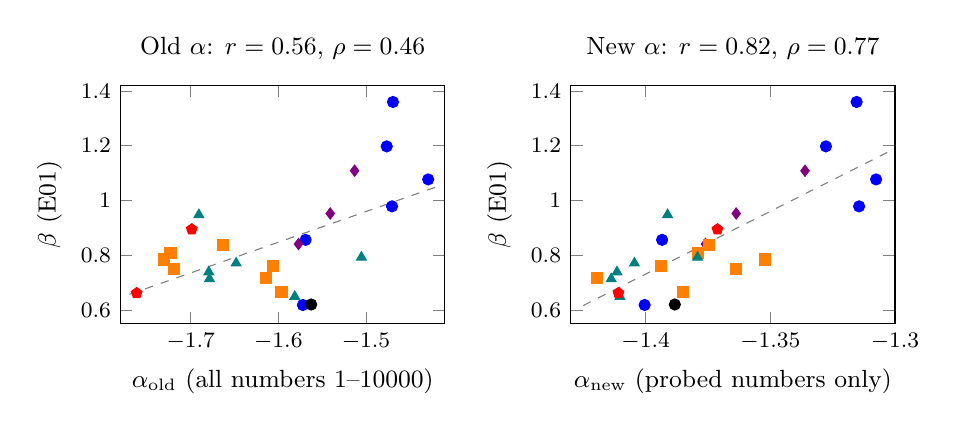
\begin{tikzpicture}
\begin{groupplot}[group style={group size=2 by 1, horizontal sep=1.6cm},
  width=0.47\textwidth, height=0.38\textwidth, ylabel={$\beta$ (E01)},
  ymin=0.55, ymax=1.42, tick label style={font=\footnotesize}, label style={font=\small},
  title style={font=\small}, legend style={font=\footnotesize, draw=none, fill=none},
  legend cell align=left]
\nextgroupplot[xlabel={$\aold$ (all numbers 1--10000)}, title={Old $\alpha$: $r=0.56$, $\rho=0.46$},
  xmin=-1.78, xmax=-1.41, legend to name=famlegend, legend columns=7,
  legend style={/tikz/every even column/.append style={column sep=6pt}}]
\addplot[domain=-1.77:-1.42, gray, dashed] {2.6395 + 1.1200*x}; \addlegendentry{fit}
\addplot[only marks, mark=*, blue] coordinates {(-1.4692,1.3595) (-1.4763,1.1974) (-1.4290,1.0768) (-1.4703,0.9784) (-1.5689,0.8561) (-1.5720,0.6183)}; \addlegendentry{Dolma}
\addplot[only marks, mark=diamond*, violet] coordinates {(-1.5130,1.1085) (-1.5408,0.9523) (-1.5770,0.8409)}; \addlegendentry{DCLM+Dolma}
\addplot[only marks, mark=square*, orange] coordinates {(-1.6634,0.8381) (-1.7230,0.8091) (-1.7307,0.7841) (-1.6060,0.7601) (-1.7193,0.7501) (-1.6142,0.7172) (-1.5965,0.6655)}; \addlegendentry{DCLM}
\addplot[only marks, mark=triangle*, teal] coordinates {(-1.6907,0.9477) (-1.5052,0.7925) (-1.6482,0.7710) (-1.6794,0.7388) (-1.6786,0.7135) (-1.5813,0.6490)}; \addlegendentry{Falcon}
\addplot[only marks, mark=pentagon*, red] coordinates {(-1.6988,0.8947) (-1.7617,0.6617)}; \addlegendentry{FineWeb}
\addplot[only marks, mark=otimes*, black] coordinates {(-1.5625,0.6201)}; \addlegendentry{C4}
\nextgroupplot[xlabel={$\anew$ (probed numbers only)}, title={New $\alpha$: $r=0.82$, $\rho=0.77$},
  xmin=-1.43, xmax=-1.30, xticklabel style={/pgf/number format/fixed, /pgf/number format/precision=2}]
\addplot[domain=-1.425:-1.302, gray, dashed] {7.1491 + 4.5843*x};
\addplot[only marks, mark=*, blue] coordinates {(-1.3154,1.3595) (-1.3277,1.1974) (-1.3076,1.0768) (-1.3144,0.9784) (-1.3934,0.8561) (-1.4004,0.6183)};
\addplot[only marks, mark=diamond*, violet] coordinates {(-1.3361,1.1085) (-1.3637,0.9523) (-1.3760,0.8409)};
\addplot[only marks, mark=square*, orange] coordinates {(-1.3747,0.8381) (-1.3789,0.8091) (-1.3522,0.7841) (-1.3940,0.7601) (-1.3639,0.7501) (-1.4196,0.7172) (-1.3850,0.6655)};
\addplot[only marks, mark=triangle*, teal] coordinates {(-1.3912,0.9477) (-1.3792,0.7925) (-1.4045,0.7710) (-1.4115,0.7388) (-1.4138,0.7135) (-1.4103,0.6490)};
\addplot[only marks, mark=pentagon*, red] coordinates {(-1.3712,0.8947) (-1.4109,0.6617)};
\addplot[only marks, mark=otimes*, black] coordinates {(-1.3883,0.6201)};
\end{groupplot}
\end{tikzpicture}

\pgfplotslegendfromname{famlegend}
\caption{$\beta$ against the two definitions of $\alpha$; one point per model, colour = family.
With the old $\alpha$ the trend comes mostly from Dolma (blue) versus the rest; with the new $\alpha$
the web-only families also follow the trend.}
\label{fig:e11}
\end{figure}

\paragraph{Results.}
\begin{itemize}
\item With $\anew$ the relation is much stronger: $r = 0.82$ ($p<10^{-6}$), $\rho = 0.77$, with no model
  removed.
\item It does not depend on any single model (leave-one-out: $r = 0.79$--$0.84$) or family.
\item It survives removing Dolma ($r=0.68$), holds within families ($r=0.75$, vs 0.28 for $\aold$), and
  is strongest on the 8 independent base corpora ($r=0.92$).
\item The recipes are related (variants of the same corpus), so we also resampled whole families
  (family-level bootstrap): 95\% interval for $r$ is $[0.39, 0.90]$, which excludes 0. Using one
  average point per family: $r = 0.84$ ($p=0.035$, 6 points).
\item Controlling for code+math share weakens it: partial $r = 0.30$ ($p \approx 0.15$) for $\anew$,
  $-0.23$ for $\aold$. Code/math content explains part of the relation.
\end{itemize}

\paragraph{Caveats.}
\begin{itemize}
\item \textbf{Chosen after seeing the data.} This $\alpha$ was adopted after the original $\alpha$ was known to correlate weakly. A second natural variant
  (pooling every probed number) agrees ($r=0.79$, $\rho=0.80$). It should be reported as exploratory
  and next to $\aold$, until tested on new models.
\item Only 4 points per model, so $\anew$ is a coarse slope.
\item Without any code/math recipes the relation is positive but moderate ($\rho = 0.52$, $r = 0.44$,
  $p = 0.08$): the content confound is reduced, not removed.
\item With E06's $\beta$ at E06's own layer choices the relation is weaker ($r=0.60$), for the near-tie
  reason in E06; at E01's layers it is $r=0.77$. At a fixed layer 8 the new $\alpha$ is no better than the
  old one ($r=0.75$ for both).
\end{itemize}

\paragraph{What it addresses.} Sensitivity to individual corpora, leave-one-out, the influence of
Dolma, analysis by family, and uncertainty (VRQv Q2, H7EL, a1nj Q1). It also explains \emph{why} the
original $\alpha$ is weak: it measures mostly numbers $\beta$ does not probe.

%% ===================================================================
\clearpage
\section*{Appendix: all 25 models}

\begin{table}[h]
\centering\footnotesize
\caption{Per-model values, sorted by $\beta$. Layer and Order from E01; $\beta$ (E01) $\pm$ s.d.\ over
3 prompt seeds; $\beta$ (E06) = 10-group smooth fit at the same layer. $^{*}$Recipe contains code or
math documents.}
\label{tab:all}
\begin{tabular}{@{}llcc ccc c@{}}
\toprule
Model & Family & Layer & Order & $\beta$ (E01) & $\beta$ (E06) & $\aold$ & $\anew$ \\
\midrule
\texttt{dolma1\_7-no-reddit$^{*}$} & Dolma & 8 & 0.91 & $1.36\pm0.06$ & 1.18 & $-1.47$ & $-1.315$ \\
\texttt{dolma1\_7-no-flan$^{*}$} & Dolma & 9 & 0.93 & $1.20\pm0.06$ & 1.19 & $-1.48$ & $-1.328$ \\
\texttt{dclm-baseline-25p-dolma1.7-75p$^{*}$} & DCLM+Dolma & 8 & 0.93 & $1.11\pm0.06$ & 1.10 & $-1.51$ & $-1.336$ \\
\texttt{dolma1\_6plus$^{*}$} & Dolma & 9 & 0.92 & $1.08\pm0.06$ & 1.01 & $-1.43$ & $-1.308$ \\
\texttt{dolma1\_7$^{*}$} & Dolma & 6 & 0.93 & $0.98\pm0.08$ & 0.92 & $-1.47$ & $-1.314$ \\
\texttt{dclm-baseline-50p-dolma1.7-50p$^{*}$} & DCLM+Dolma & 8 & 0.95 & $0.95\pm0.05$ & 0.83 & $-1.54$ & $-1.364$ \\
\texttt{falcon-and-cc-qc-tulu-10p} & Falcon & 9 & 0.93 & $0.95\pm0.04$ & 0.81 & $-1.69$ & $-1.391$ \\
\texttt{fineweb-edu} & FineWeb & 9 & 0.96 & $0.89\pm0.04$ & 0.87 & $-1.70$ & $-1.371$ \\
\texttt{dolma1\_7-no-code$^{*}$} & Dolma & 8 & 0.94 & $0.86\pm0.06$ & 0.77 & $-1.57$ & $-1.393$ \\
\texttt{dclm-baseline-75p-dolma1.7-25p$^{*}$} & DCLM+Dolma & 10 & 0.94 & $0.84\pm0.07$ & 0.76 & $-1.58$ & $-1.376$ \\
\texttt{dclm-baseline-qc-7p-fw2} & DCLM & 8 & 0.95 & $0.84\pm0.04$ & 0.67 & $-1.66$ & $-1.375$ \\
\texttt{dclm-baseline-qc-fw-10p} & DCLM & 3 & 0.94 & $0.81\pm0.03$ & 0.76 & $-1.72$ & $-1.379$ \\
\texttt{falcon} & Falcon & 9 & 0.92 & $0.79\pm0.05$ & 0.68 & $-1.51$ & $-1.379$ \\
\texttt{dclm-baseline-qc-fw-3p} & DCLM & 9 & 0.93 & $0.78\pm0.00$ & 0.57 & $-1.73$ & $-1.352$ \\
\texttt{falcon-and-cc-qc-orig-10p} & Falcon & 8 & 0.94 & $0.77\pm0.06$ & 0.66 & $-1.65$ & $-1.405$ \\
\texttt{dclm-baseline-qc-20p} & DCLM & 9 & 0.95 & $0.76\pm0.06$ & 0.72 & $-1.61$ & $-1.394$ \\
\texttt{dclm-baseline-qc-7p-fw3} & DCLM & 9 & 0.92 & $0.75\pm0.08$ & 0.60 & $-1.72$ & $-1.364$ \\
\texttt{falcon-and-cc-qc-20p} & Falcon & 8 & 0.93 & $0.74\pm0.06$ & 0.68 & $-1.68$ & $-1.411$ \\
\texttt{dclm-baseline-qc-10p} & DCLM & 8 & 0.93 & $0.72\pm0.06$ & 0.66 & $-1.61$ & $-1.420$ \\
\texttt{falcon-and-cc-qc-10p} & Falcon & 8 & 0.92 & $0.71\pm0.07$ & 0.60 & $-1.68$ & $-1.414$ \\
\texttt{dclm-baseline} & DCLM & 8 & 0.90 & $0.67\pm0.07$ & 0.58 & $-1.60$ & $-1.385$ \\
\texttt{fineweb-pro} & FineWeb & 7 & 0.93 & $0.66\pm0.01$ & 0.58 & $-1.76$ & $-1.411$ \\
\texttt{falcon-and-cc} & Falcon & 9 & 0.93 & $0.65\pm0.04$ & 0.63 & $-1.58$ & $-1.410$ \\
\texttt{c4} & C4 & 7 & 0.93 & $0.62\pm0.05$ & 0.57 & $-1.56$ & $-1.388$ \\
\texttt{dolma1\_7-no-math-code} & Dolma & 4 & 0.94 & $0.62\pm0.04$ & 0.55 & $-1.57$ & $-1.400$ \\
\bottomrule
\end{tabular}
\end{table}

\end{document}
